% ============================================================
% Seccion: Explicacion del tema
% Problema, motivacion, objetivos y estado del arte
% ============================================================
\section{Tema de estudio}

% ============================================================
\begin{frame}
\frametitle{Problema y motivación}
\vspace{-0.6em}
{\small
\begin{itemize}\itemsep=3pt
\item \textbf{Curva de luz}: brillo de una estrella en el tiempo. En una estrella periódica
  se repite cada cierto \textbf{período}
\item \textbf{ALeRCE} procesa las alertas del survey ZTF y resume cada curva en
  \textbf{178 features}: período, amplitud, color, etc.
\item \textbf{Problema}: 178 números por estrella no se pueden inspeccionar a ojo. Se necesita un
  espacio de pocas dimensiones donde aparezcan grupos y se distingan los objetos raros
\item \textbf{Motivación}: los surveys generan más alertas de las que se pueden revisar a mano,
  y los objetos que no calzan con ninguna clase conocida son los de mayor interés
\end{itemize}
}
\vspace{-0.3em}
\begin{center}
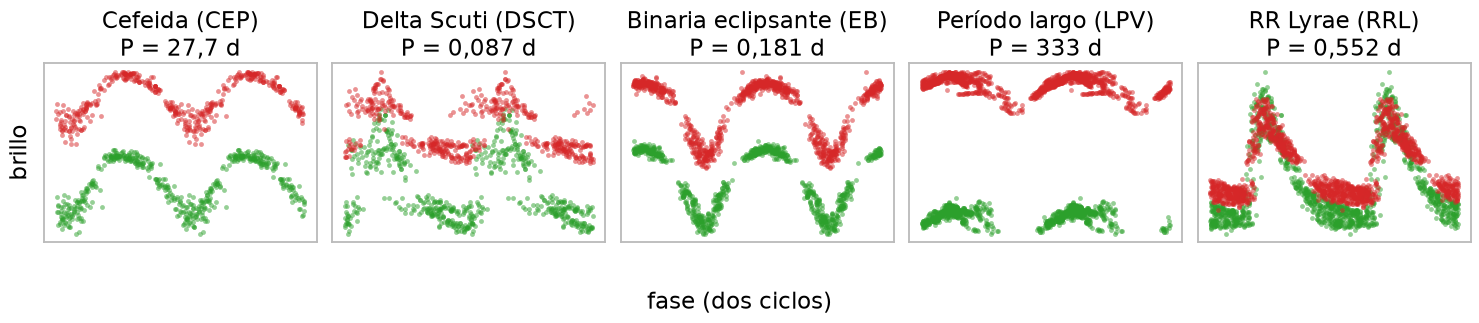
\includegraphics[width=0.86\textwidth]{figures/clases_curvas.png}\\[-0.2em]
{\scriptsize Las cinco clases del proyecto: curva plegada de un objeto típico de cada una
\quad$\cdot$\quad
\textcolor{green!55!black}{$\blacksquare$} banda g \quad \textcolor{red!80!black}{$\blacksquare$} banda r}
\end{center}
\end{frame}

% ============================================================
\begin{frame}
\frametitle{Objetivos y estado del arte}
\vspace{-0.5em}
\begin{columns}[T]
\begin{column}{0.50\textwidth}
{\small \textbf{Objetivo general}}
\vspace{0.2em}

{\footnotesize Agrupar estrellas variables periódicas de ALeRCE--ZTF en el espacio latente de un
autoencoder, y analizar los grupos y los posibles outliers a partir de sus curvas de luz.}

\vspace{0.7em}
{\small \textbf{Etapas del proyecto}}
\vspace{0.1em}
{\footnotesize
\begin{enumerate}\itemsep=3.5pt
\item Exploración preliminar de los datos con visualizaciones (UMAP, t-SNE, \emph{corner plots})
\item Visualización con autoencoders: cuello de botella de 2 dimensiones o más
\item Clustering con mezcla de gaussianas (GMM) y Multi-Class Deep SVDD sobre el cuello de botella
\item Visualización de las curvas de luz de los clusters y análisis de outliers
\end{enumerate}
}
\end{column}

\begin{column}{0.47\textwidth}
{\small \textbf{Estado del arte}}
\vspace{0.1em}
{\footnotesize
\begin{itemize}\itemsep=4.5pt
\item \textbf{ALeRCE} {\color{gray}(Förster et al.\ 2021)}: broker que clasifica alertas de ZTF.
  Su clasificador de curvas de luz usa las features de este proyecto
  {\color{gray}(Sánchez-Sáez et al.\ 2021)}
\item \textbf{DAGMM} {\color{gray}(Zong et al.\ 2018)}: autoencoder más mezcla de gaussianas en el
  espacio latente. Una verosimilitud baja marca la anomalía
\item \textbf{Deep SVDD} {\color{gray}(Ruff et al.\ 2018)}: un encoder que contrae los datos
  normales alrededor de un centro
\item \textbf{Multi-Class Deep SVDD} {\color{gray}(Pérez-Carrasco et al.\ 2023)}: un centro por
  clase conocida. Es el detector de anomalías de ALeRCE
\end{itemize}
}
\end{column}
\end{columns}
\end{frame}
